\chapter{Wykorzystane technologie}

\section{Xcode i Developer Tools}
Xcode jest IDE (Integrated development environment) stworzonym przez Apple i dostępnym za darmo do pobrania z App Store, sklepu
z aplikacjami do którego dostęp mają wyłącznie użytkownicy komputerów z systemem MacOS. Jest wyposażony w pakiet wszystkich narzędzi
(Developer Tools) potrzebnych dla developerów aby tworzyć aplikacje na iOS. Główną aplikacją pakietu jest Xcode IDE który wraz z
wspomagającymi aplikacjami dostępnymi w pakiecie takimi jak Simulator czy Instruments czyni pracę przy tworzeniu aplikacji płynną
i efektowną. W tym rozdziale przedstawię właśnie te narzędzia ze względu na ich rolę w procesie tworzenia aplikacji.

\begin{figure}[ht!]
  \centering
  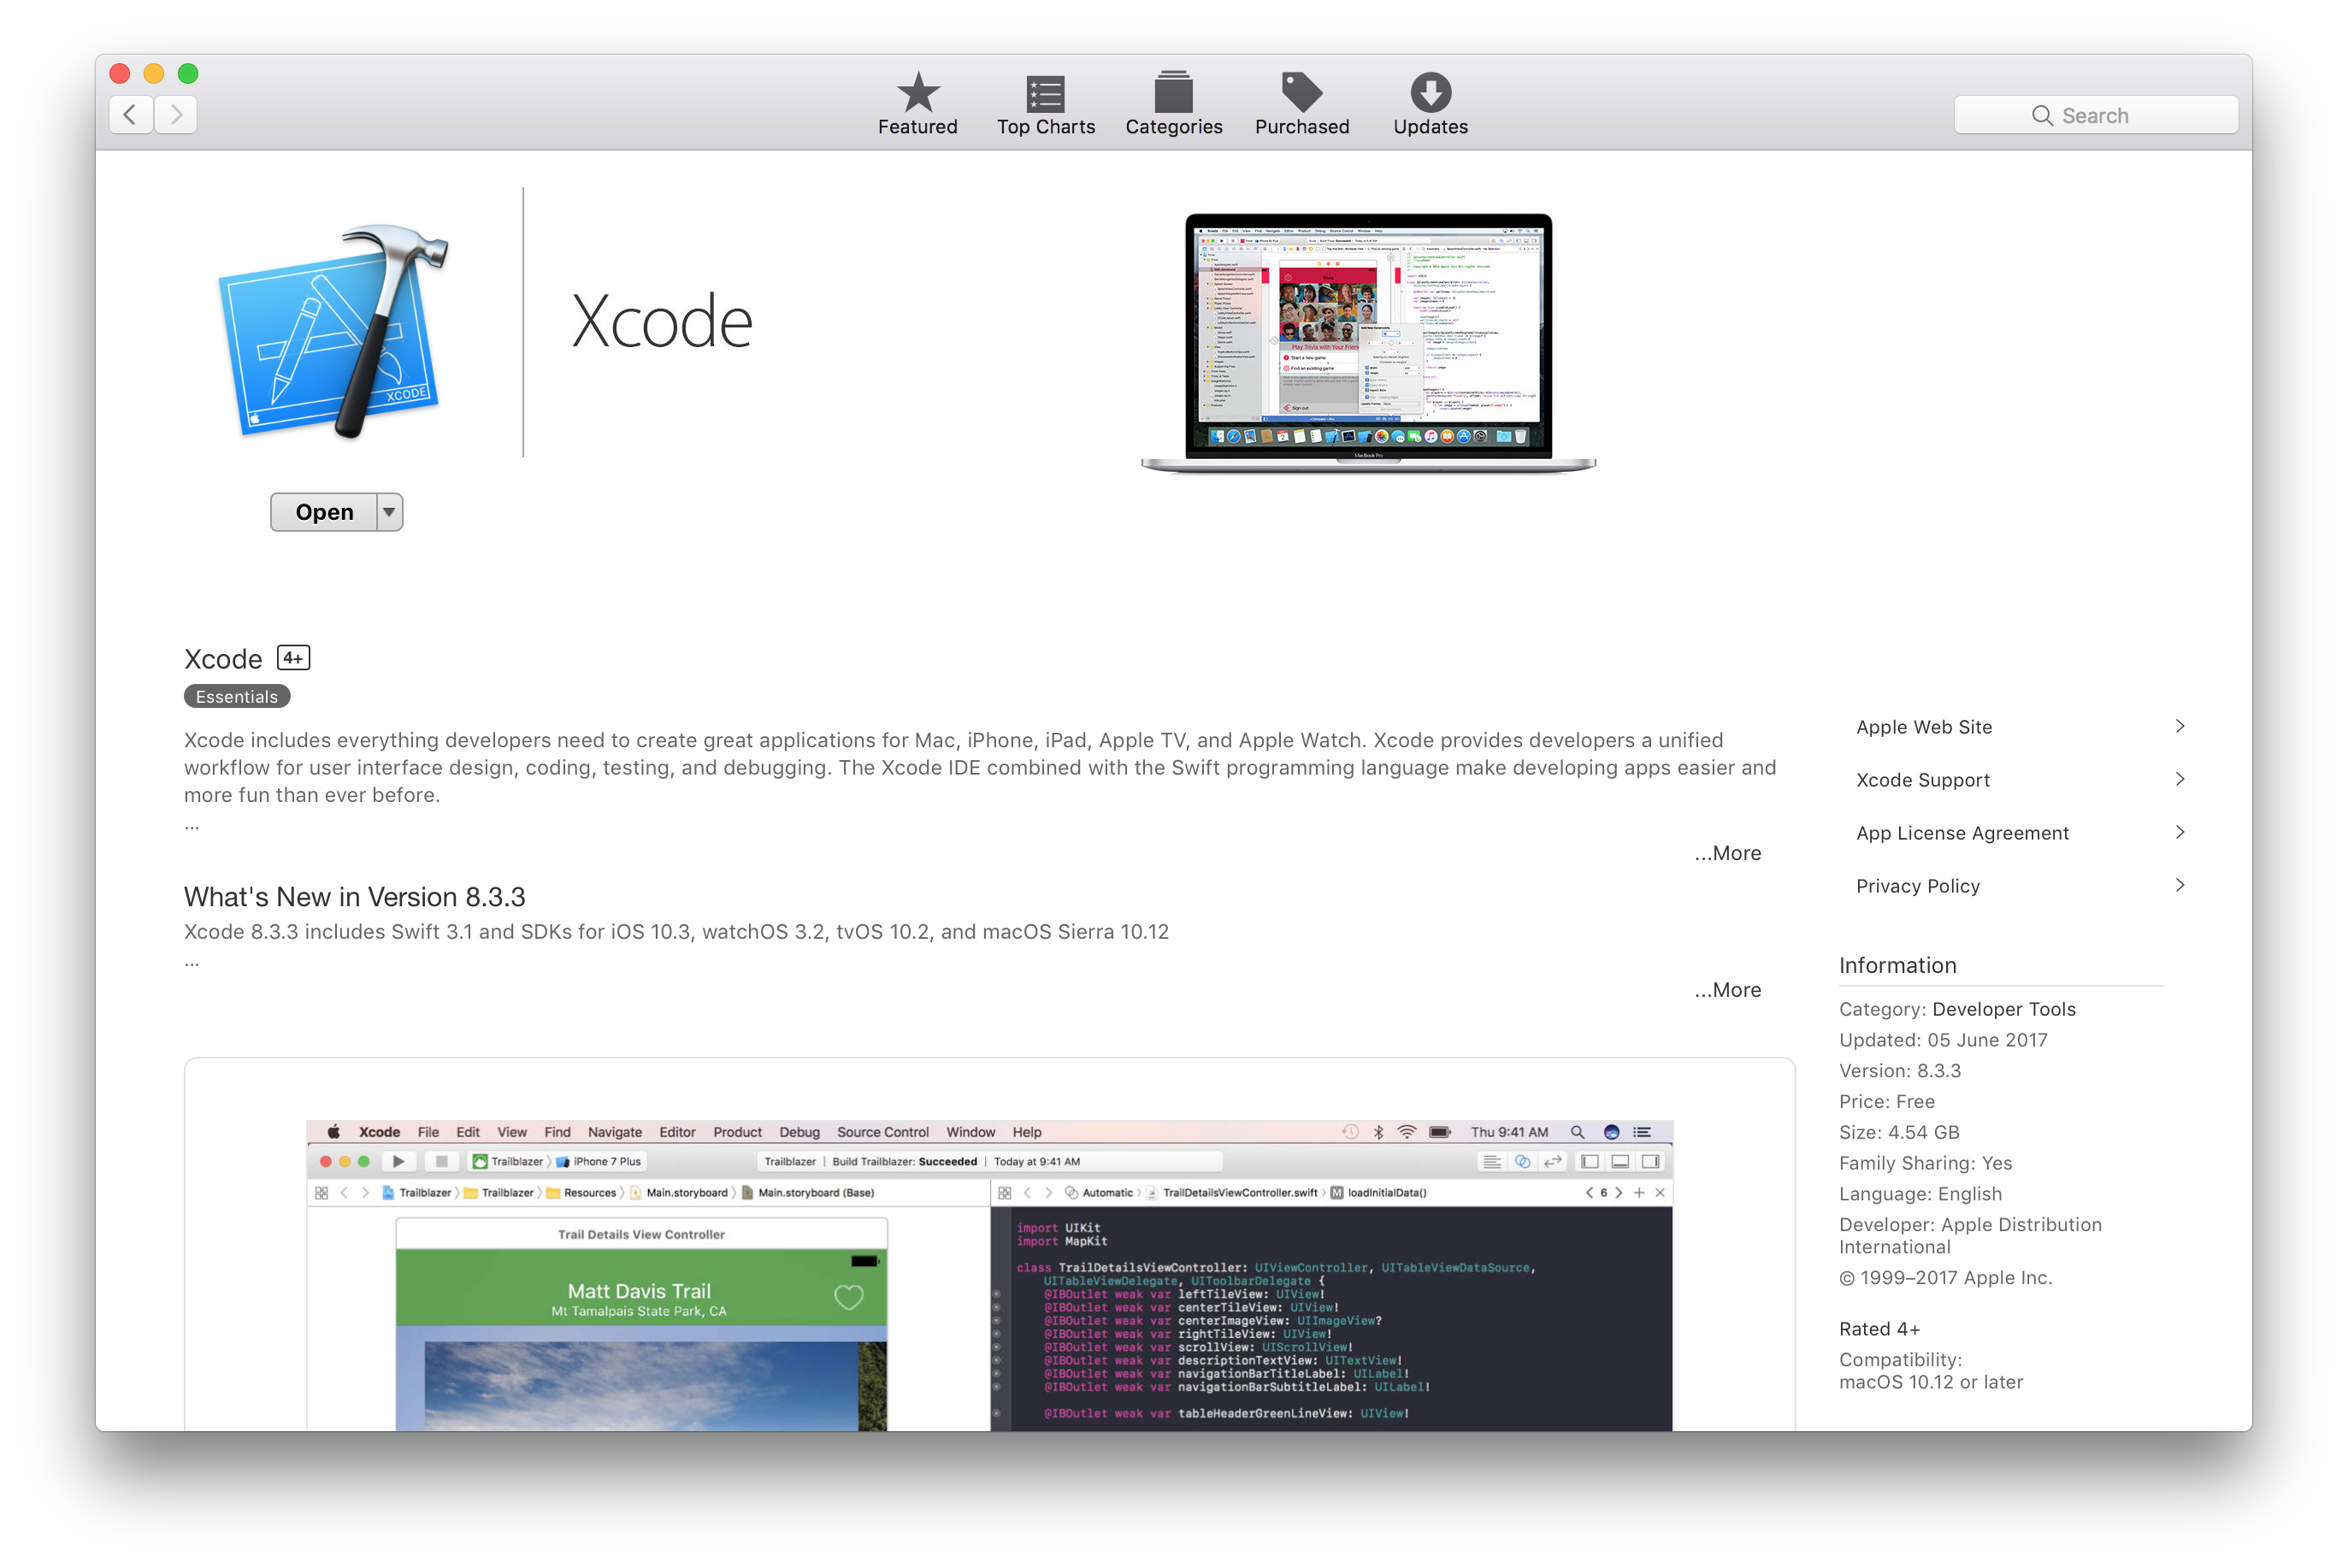
\includegraphics[width=120mm]{images/chapter-2-image-1-appstore.png}
  \caption{Xcode w App Store}
  \label{overflow}
\end{figure}

\paragraph{Xcode IDE}

Xcode jako nowoczesne, produktywne środowisko jest miejscem w którym programista aplikacji na iOS spędza znaczną większość swojego
czasu. Całość prac wykonywanych przy produkcji aplikacji może zostać wykonana właśnie tutaj. Najbardziej podstawowy element jakim
jest edytor tekstu dobrze współgra z takimi narzędziami jak Interface Buildier, który pozwala w prosty sposób zaprojektować stronę
wizualną aplikacji przy użyciu Storyboardów a następnię stworzyć referencję w kodzie do wybranych przez nas elementów przez proste
przeciągnięcie myszką. Storyboardy są opcjonalnym aczkolwiek bardzo pożytecznym narzędziem szczególnie dla programistów stawiających
swoje pierwsze kroki na tej platformie. Zapewniają one wizualne wyobrazenie interfejsu aplikacji nad którą wykonywana jest praca,
a projektowanie dowolnego widoku który będzie wyglądał dobrze na każdym urządzeniu w dowolnej orientacji, jest relatywnie proste po
zapoznaniu się z kilkoma elementarnymi zasadami.

\begin{figure}[ht!]
  \centering
  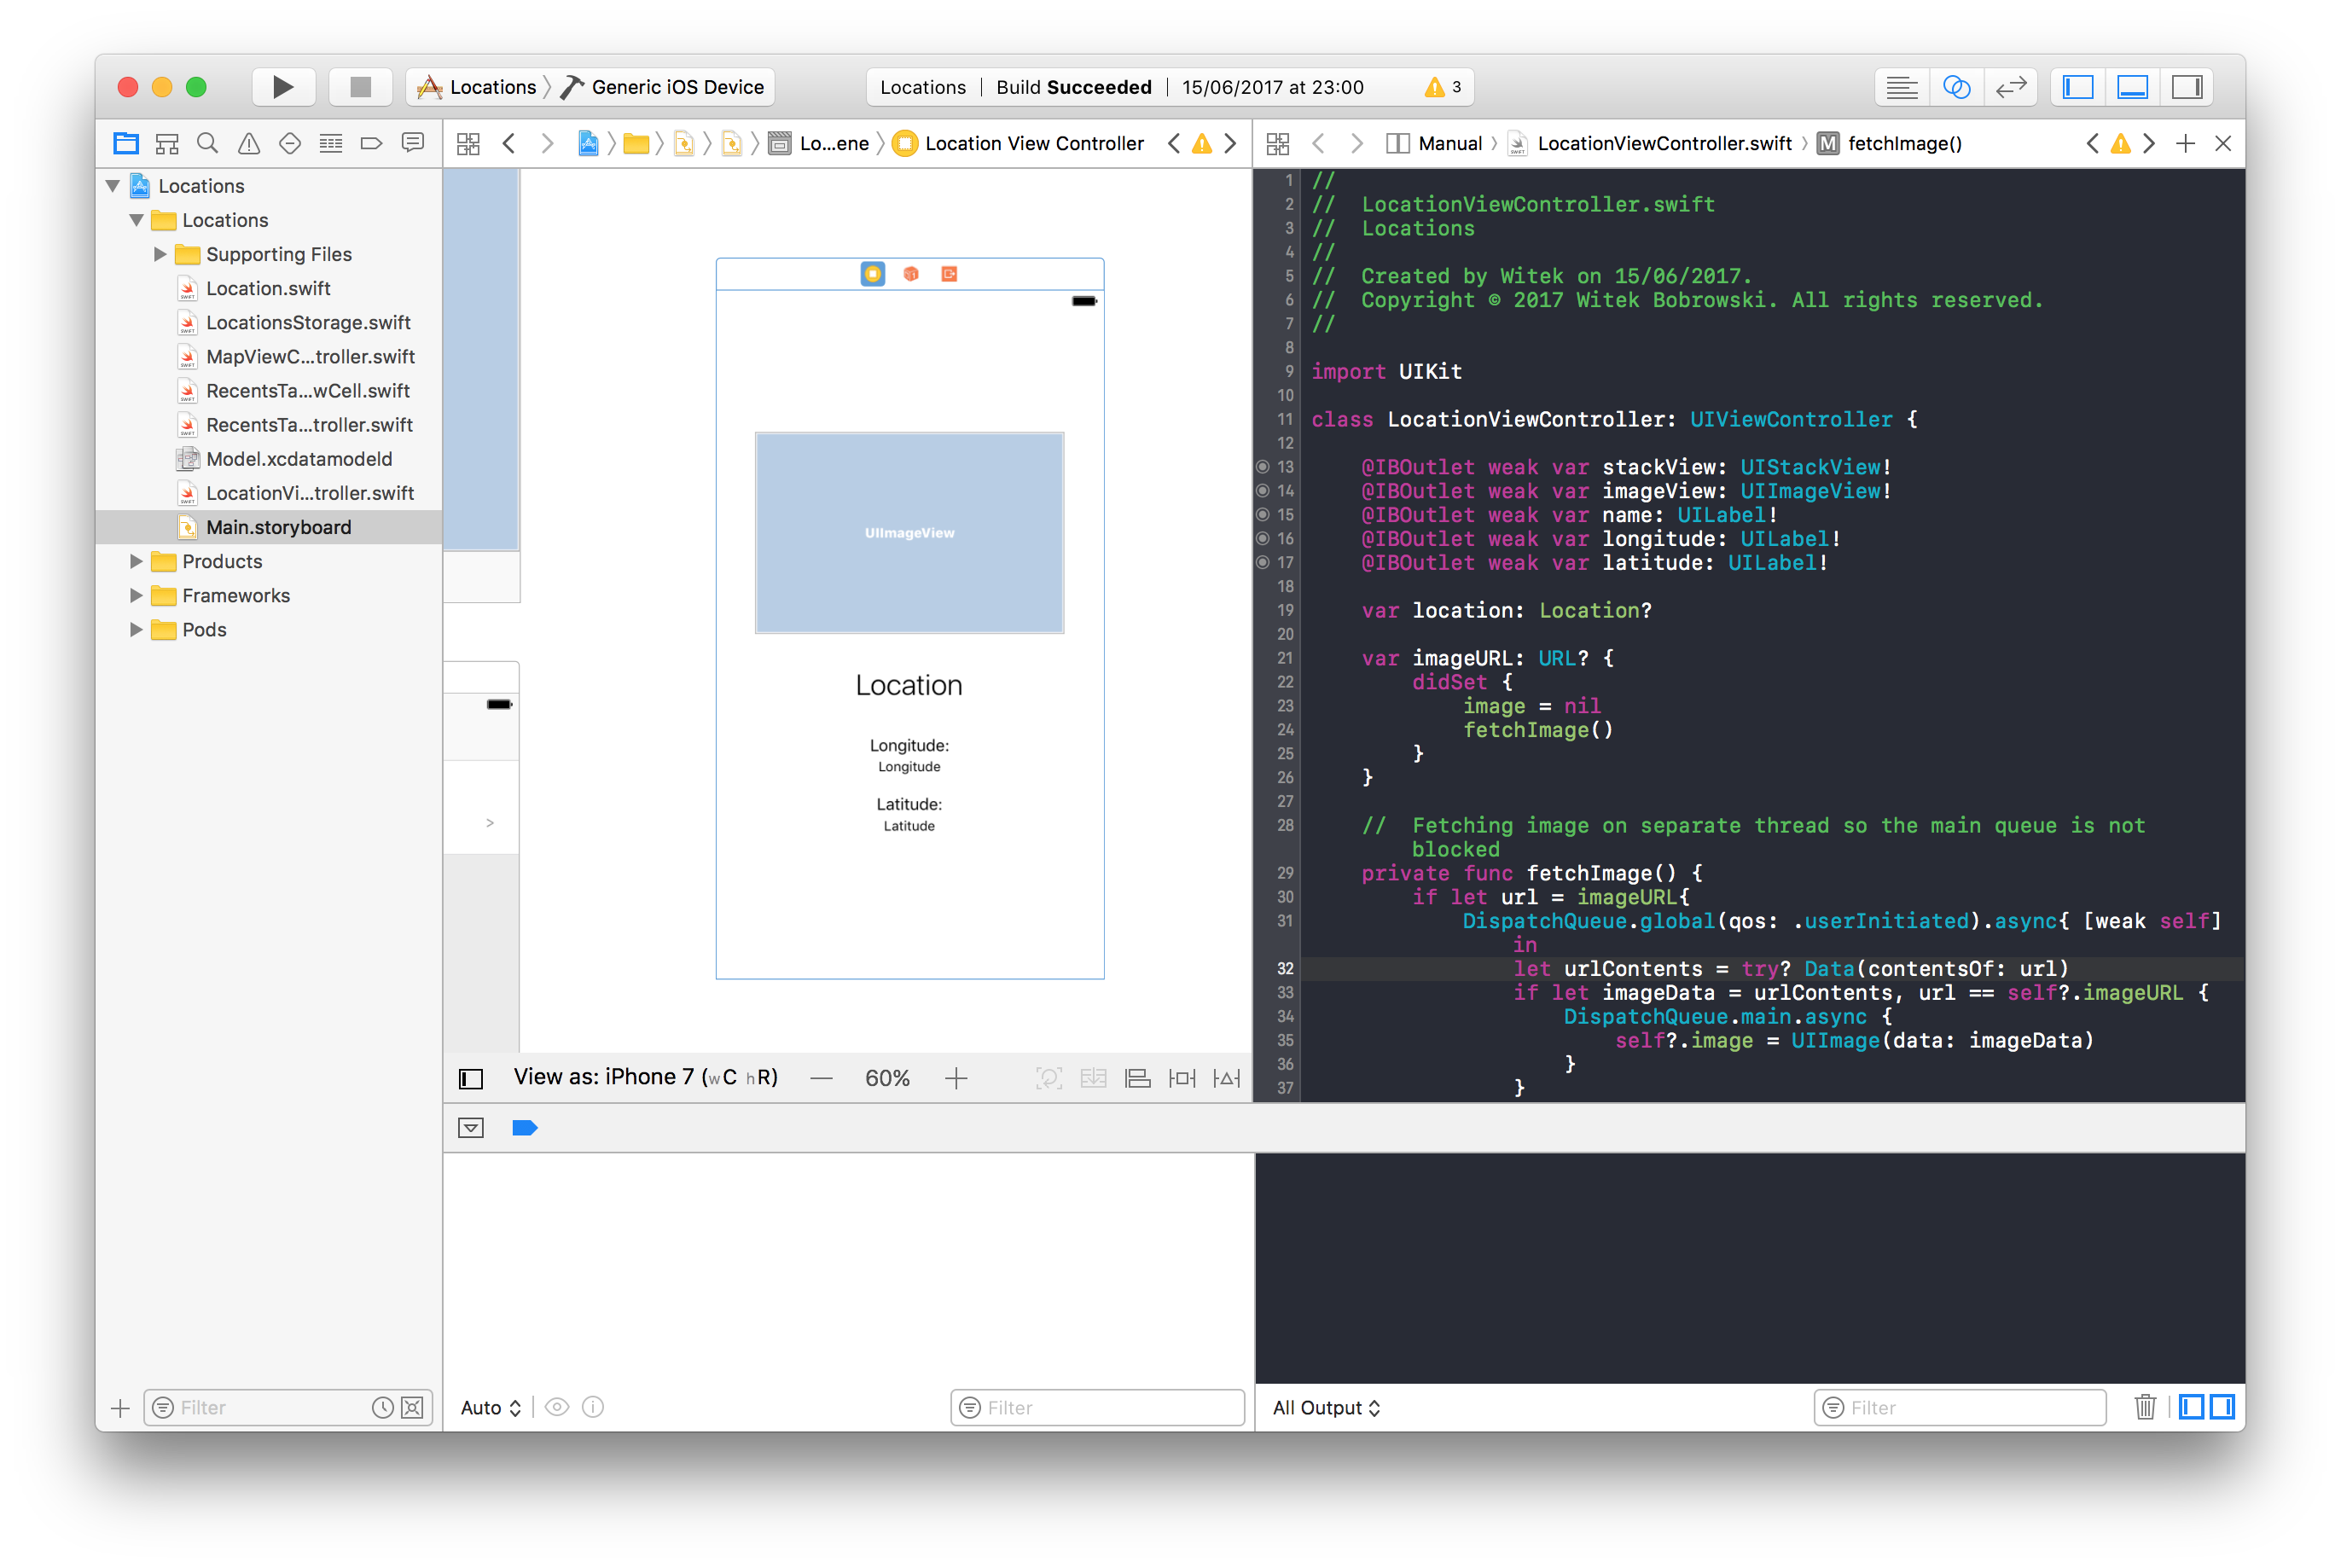
\includegraphics[width=120mm]{images/chapter-2-image-2-xcode.png}
  \caption{Xcode pokazujący "Assistant editor"}
  \label{overflow}
\end{figure}

Ponieważ Storyboardy tworzy się w jednym pliku o formacie .storyboard, często w profesjonalnej produkcji rezygnuje się z nich ze
względu na konflikty w systemach kontrolii wersji. Konflikty te powstają w wyniku pracy wielu programistów, a ponieważ plik .storyboard
jest w rzeczywistości plikiem XML, który został wygenerowany automatycznie, rozwiązywanie konfilków bywa kłopotliwe, a przy dużych
projektach problematyczne. Dlatego rezygnuje się z nich na rzecz tworzenia widoków tylko przy użyciu kodu, oraz niezależnych plików XIB.
Pliki te pozwalają na ustawienie elementów w stylu znanym ze Storyboardów lecz w przeciwieństwie do nich reprezentrują pojedyńczy widok,
dzięki czemu problem z konfliktami zostaje uniknięty a jednocześnie tworzenie bardziej skomplikowanych widoków pozostaje znacznie
ułatwione.

Xcode zapewnia wsparcie dla systemu kontroli wersji git. Przy tworzeniu nowego projektu, gdy jest o to poproszony, inicjalizuje nowe
repozytorium. Dodatkowo w nawigatorze projektu, w którym widać strukturę projektu, Xcode oznaczy literą "M" pliki które git oznacza
jako pliki w których dokonano zmian (modified) a literą "A" (add) pliki które zostały dodane od czasu poprzedniego zachowania zmian.
W najnowszej wersji 9.0, Xcode zyskał nową funkcjonalność - Source Control Navigator, który pozwala na eksplorowanie poszczególnych
gałęzi repozytorium i podglądu dowolnego momentu w historii repozytorium. 

\paragraph{Simulator}

\paragraph{Instruments}

\section{Swift}

\section{iOS SDK}

\section{Zewnętrzne biblioteki}
